\chapter{Implementacja systemu}
	Ostateczna forma projektu przedstawiona została przy pomocy diagramów UML, wygenerowanych autorskim skryptem na podstawie kodu źródłowego gotowego programu.

\section{Warstwa rdzeniowa}
	W warstwie rdzeniowej ujęte zostały najczęściej używane struktury z pakietu Direct3D 11. Wrappery takich obiektów zostały oznaczone prefixem D3D. Pozostałe klasy posiadają nazwę bez przedrostków.

\subsection{Core}
	Klasa będąca podstawą funkcjonowania całego modułu. 
	Odpowiada za tworzenie oraz zarządzanie podstawowych zasobów używanych przez aplikacje oparte o Direct3D, takich jak Device, Context, RenderTarget(View), Swap Chain czy Framebuffer. Przy jego pomocy możliwy jest wybór trybu rysowania z listy reprezentowanej przez enum PrimitiveTopologies.
	Moduł zawiera także przez kompozycję odniesienie do obiektu klasy \textbf{Window}, która zawiera w sobie logikę odpowiedzialną za zarządzanie uchwytem do systemowego okna (i zasobami z tym związanymi) oraz odpowiedziami na zmianę jego stanu i rozmiaru.
	Inicjalizacja obu elementów odbywa się przez przekazanie w konstruktorze obiektu \textbf{WindowCreationParams}, zawierającego podstawowe informacje o tworzonym oknie.
	Diagram UML przedstawiony został na rys. \ref{UML_D3DCore}.
	
	
	\begin{figure}[ht!]
		\centering
		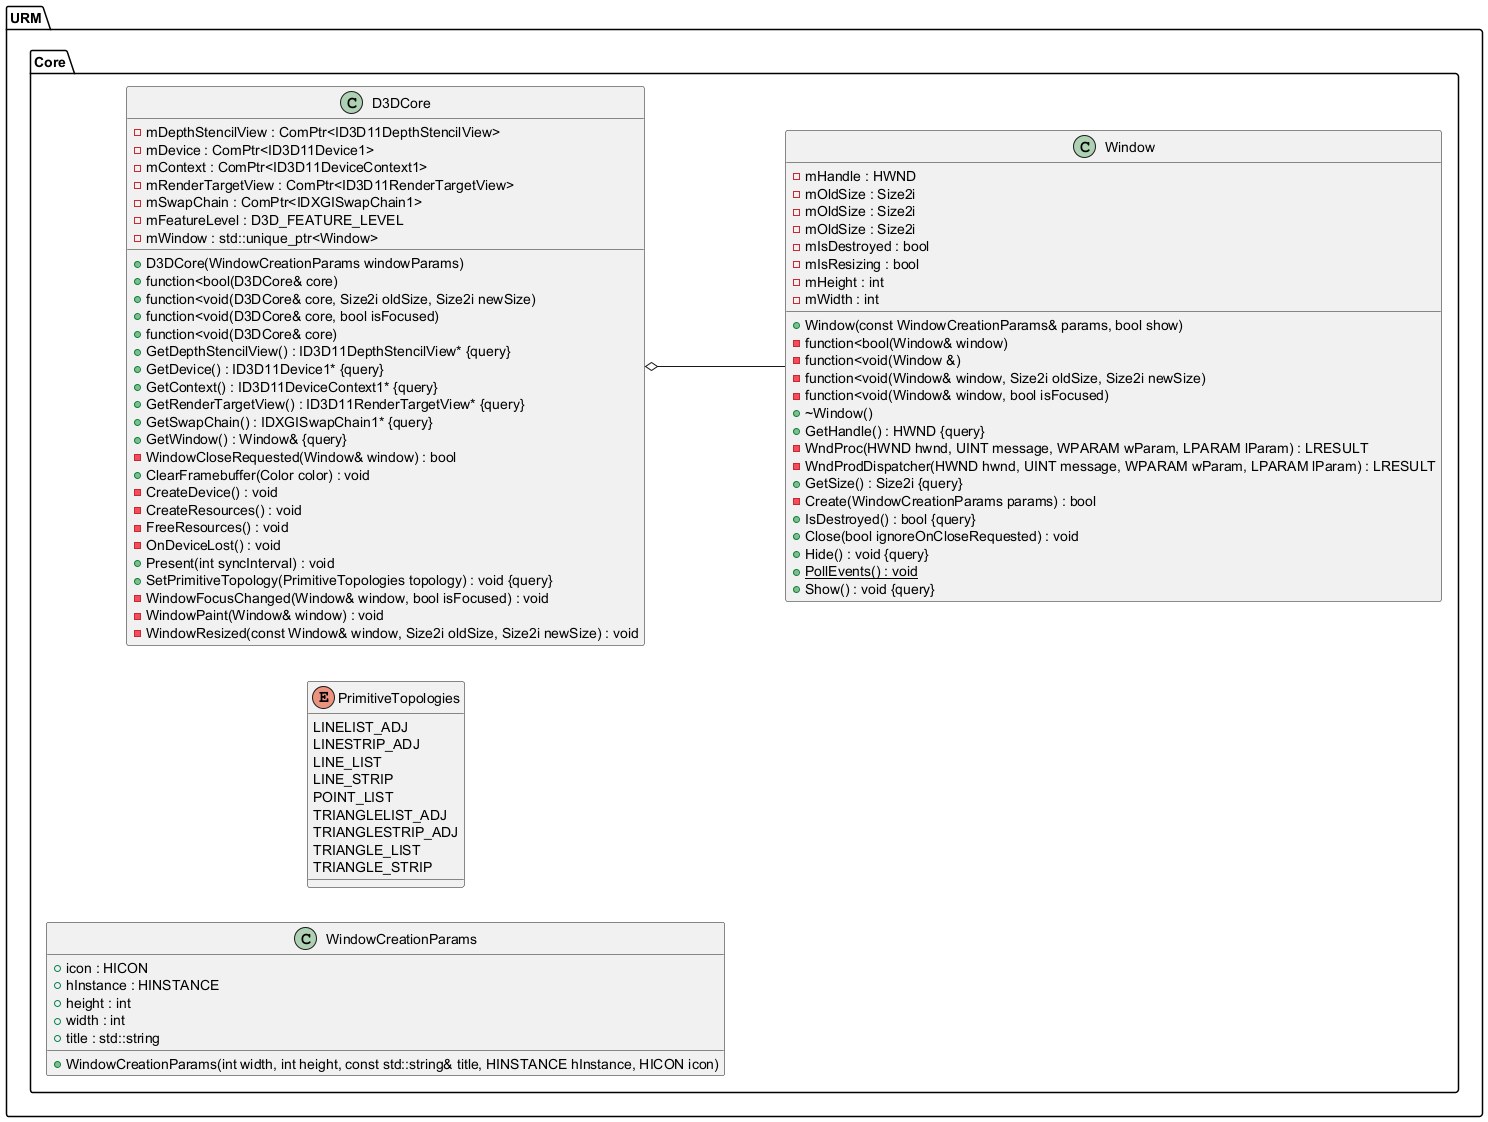
\includegraphics[width=\textwidth]{images/UML/core.png}
		\caption{Diagram UML przedstawiający kompozycję modułów D3DCore oraz Window wraz z zależnościami.}
		\label{UML_D3DCore}
	\end{figure}
	
	\vfill
	\clearpage
	
\subsection{Dziennik (Log)}
	Do prowadzenia dziennika \textit{(logu)} aktywności wykorzystana została otwartoźródłowa biblioteka \textbf{spdlog} na otwartej licencji MIT \cite{github:spdlog:spdlog}. Dodatkowo do modułu dołączona została statyczna klasa Logger opisana na rys. \ref{UML_Logger}. Udostępnia ona funkcje konfigurujące spdlog pod potrzeby projektu oraz metodę zwracającą referencję do dziennika zdarzeń krytycznych.
	

	\begin{figure}[h!]
		\centering
		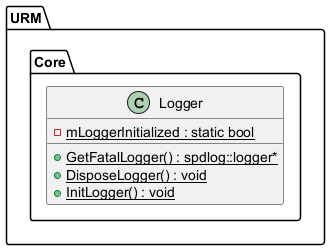
\includegraphics[width=\textwidth]{images/UML/logging.png}
		\caption{Schemat pomocniczej klasa statycznej dziennika.}
		\label{UML_Logger}
	\end{figure}
	
	\vfill
	\clearpage
	
\subsection{Metody pomocnicze}
	Sekcja zawierająca klasy i struktury pomocnicze wykorzystywane w ramach modułów projektu, przedstawione na rys. \ref{UML_Utils}.
	
	W ramach tego segmentu zaimplementowane zostały następujące klasy:
	\begin{itemize}
		\item \textbf{Size2i}: Prosta struktura opisująca rozmiar w przestrzeni 2D. Używana na przykład do określania wielkości okna.
		\item \textbf{TypeUtils}: Funkcje pomocnicze pobierania informacji o typach. Wykorzystywana między innymi do porównywania typów na podstawie wywołań generycznych.
		\item \textbf{StringUtils}: Odpowiedzialna za operacje tekstowe. Udostępnia funkcjonalność konwersji między zmiennymi tekstowymi jednobajtowymi \textit{(std::string)} oraz dwubajtowymi \textit{(std::wstring)}, a także pobierania nazwy folderu ze ścieżki do pliku.
		\item \textbf{FloatUtils}: Funkcjonalność ułatwiająca pracę z liczbami zmiennoprzecinkowymi. Dzięki metodom zawartym w tej klasie możliwe jest zbliżone porównywanie dwóch liczb typu float oraz określanie znaku tego typu liczb.
		\item \textbf{TimeUtils}: Wykorzystywana do testowania wydajności kodu. Pozwala na wywołanie dowolnej funkcji mierząc przy tym jej czas wykonania.
	\end{itemize}
	
	\begin{figure}[h!]
		\centering
		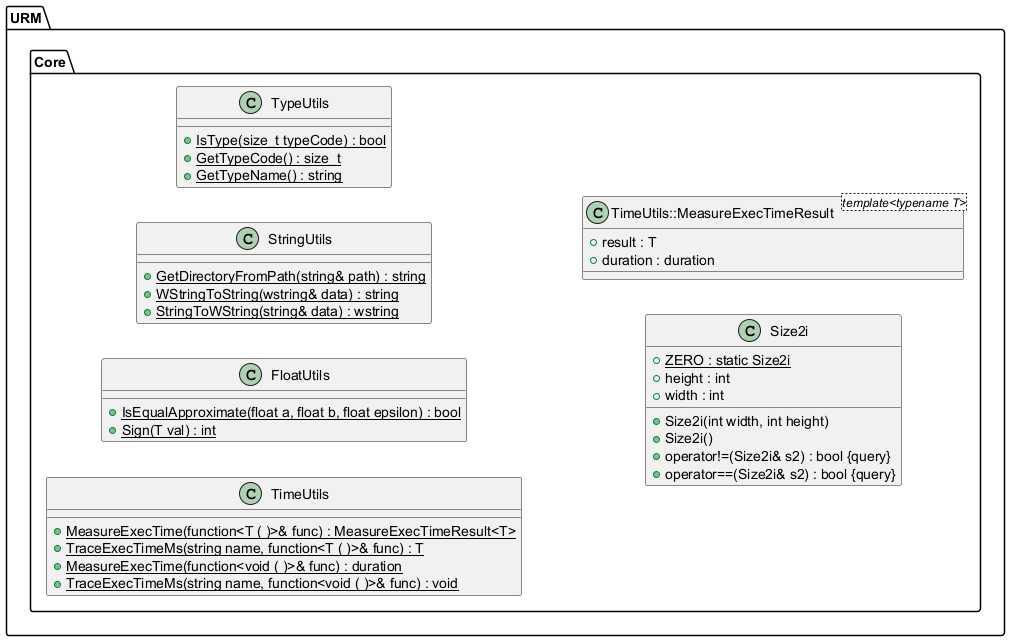
\includegraphics[width=\textwidth]{images/UML/utils.png}
		\caption{Schemat klas pomocniczych.}
		\label{UML_Utils}
	\end{figure}
	
	Do testów wydajności w trakcie oraz po zakończeniu prac nad modułem utworzona została także klasa \textbf{Stopwatch}, udostępniająca zaawansowaną funkcjonalność mierzenia czasu, a jej schemat został przedstawiony na rys. \ref{UML_Stopwatch}.
	
	\begin{figure}[h!]
		\centering
		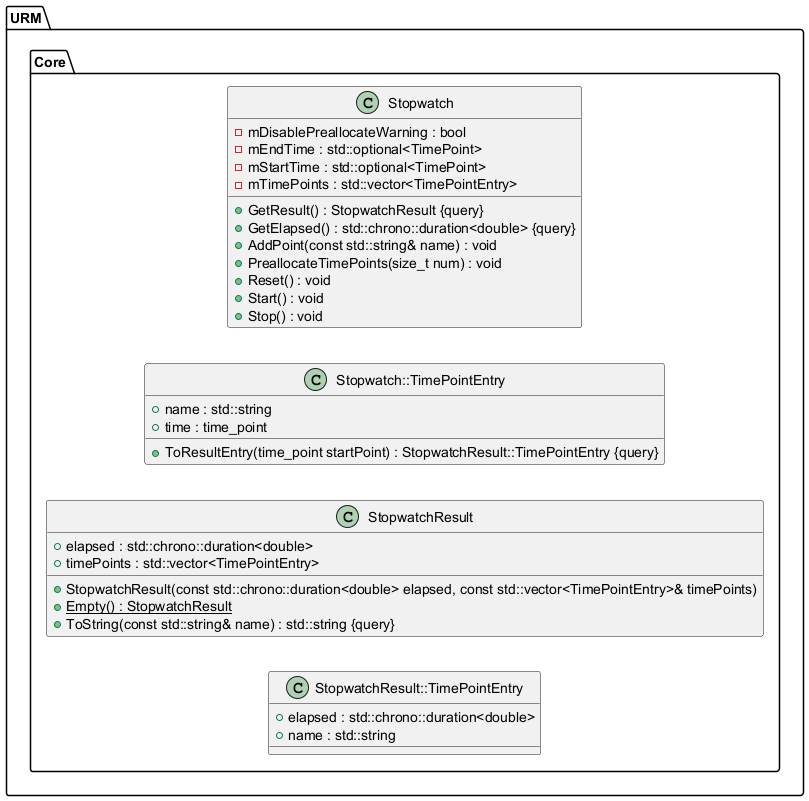
\includegraphics[width=\textwidth]{images/UML/stopwatch.png}
		\caption{Schemat klasy czasomierza.}
		\label{UML_Stopwatch}
	\end{figure}
	
\subsection{Baza D3D}
	Zbiór elementów będących warstwą abstrakcji nad niskopoziomowymi elementami pakietu Direct3D, wymaganych do jego użycia.
	\textbf{D3DViewport} odpowiedzialny jest za określanie wymiarów okna widoku (Viewport), jak i zakresu głębi rysowanego obrazu.
	Z kolei \textbf{D3DRasterizerState} pozwala na konfigurowanie parametrów procesu rasteryzacji, takich jak Culling Mode (definiowany przez enum CullModes) służący do pomijania wielokątów obróconych w złą stronę, tryb wypełnienia (przy pomocy enum FillModes), antyaliasingu, itp.
	Diagram przedstawiający strukturę opisywanych klas można zobaczyć na rys. \ref{UML_D3DUtils}
	
	\begin{figure}[h!]
		\centering
		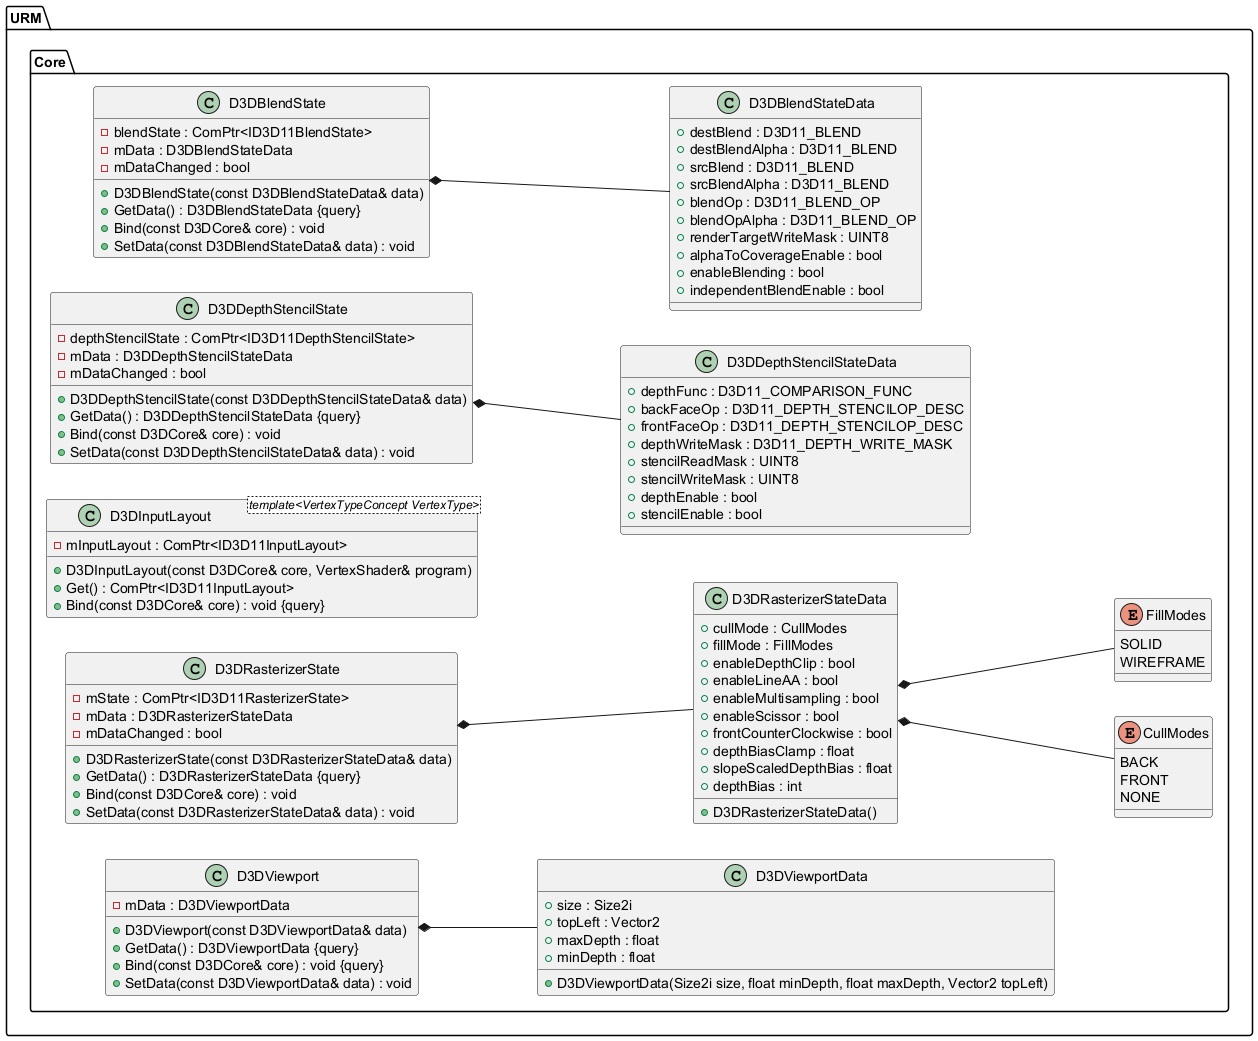
\includegraphics[width=\textwidth]{images/UML/d3dutils.png}
		\caption{Kompozycja wrapperów modułów bazowych D3D.}
		\label{UML_D3DUtils}
	\end{figure}
	
	\vfill
	\clearpage
	
\subsection{Bufory}
	Kolejnym elementem koniecznym do poprawnego korzystania z API D3D są bufory, używane jako środek przesyłu danych 
	Do ich łatwiejszej obsługi utworzona została klasa abstrakcyjna \textbf{ID3DBuffer}, której implementacje, \textbf{D3DVertexBuffer}, \textbf{D3DIndexBuffer} oraz \textbf{D3DConstantBuffer} stanowią rozwiązania do wykorzystania odpowiednio buforów wierzchołków, indeksów oraz stałych, a ich kompozycja została pokazana na rys. \ref{UML_Buffer}
	Niektóre typy parametrów zostały pominięte na diagramie w celu poprawy czytelności.
	Metoda \textit{Bind()} służy do ustawienia opisywanego przez obiekt obiektu jako aktywnego, a przy pomocy \textit{UpdateWithData(core, data)} możliwe jest zaktualizowanie danych zawartych w buforze.
		
	\begin{figure}[h!]
		\centering
		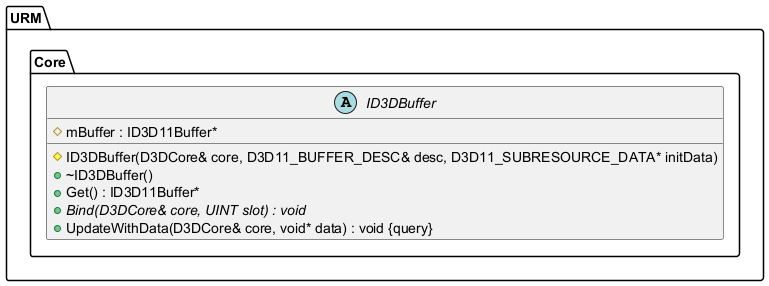
\includegraphics[width=\textwidth]{images/UML/buffer.png}
		\caption{Klasa ID3DBuffer oraz jej implementacje.}
		\label{UML_Buffer}
	\end{figure}
	
\subsection{Mesh i typy wierzchołków}
\label{SSMeshVertexTypeConcept}
	Zbiór połączonych wielokątów wraz z opisującymi go metadanymi nazywany jest Mesh'em, którego schemat przedstawiony został na rys. \ref{UML_Mesh}.
	
	Zgodnie z założeniami projektu i ten element został zaprojektowany w modularnej formie. Wykorzystując szablon typów pozwala na pracę z różnymi typami wierzchołków. Kilka typów standardowych zostało zaimplementowanych w ramach modułu \textbf{StandardVertexTypes}, opisanego na diagramie \ref{UML_VertexTypes}.
	
	\begin{figure}[h!]
		\centering
		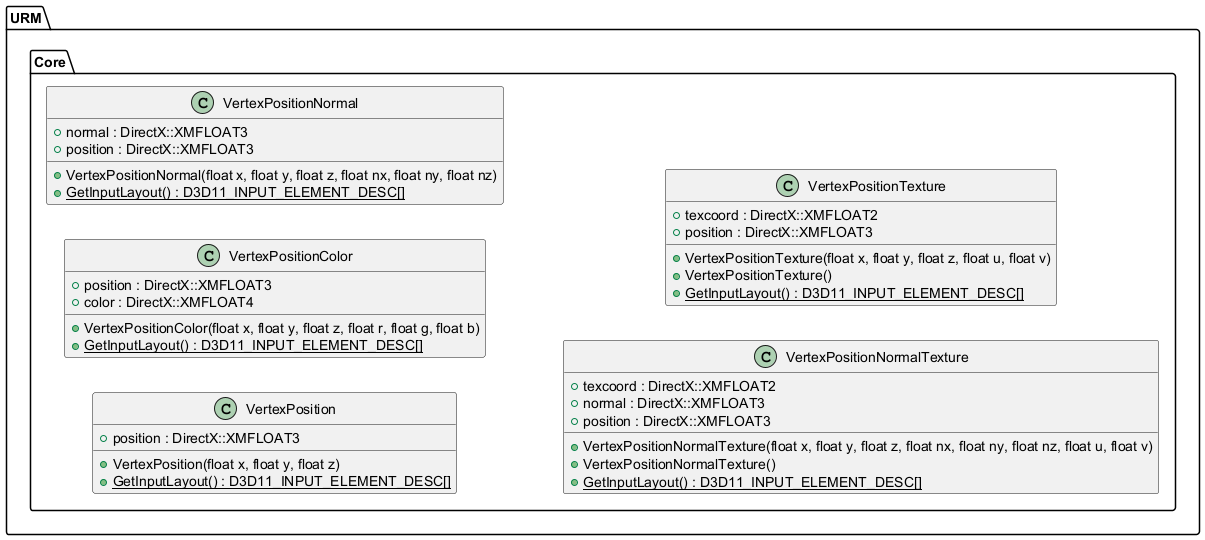
\includegraphics[width=\textwidth]{images/UML/vertextypes.png}
		\caption{Zaimplementowane standardowe typy wierzchołków.}
		\label{UML_VertexTypes}
	\end{figure}
	
	Do obsługi pozostałych typów wykorzystany został mechanizm \textit{concepts}, dodany w ramach standardu C++20 \cite{cpp20:concepts:2025}.
	Pozwala on na zdefiniowanie ograniczeń dla typu, co w opisywanym przypadku zostało wykorzystane do narzucenia konieczności implementacji statycznej metody \textit{std::vector<D3D11\_INPUT\_ELEMENT\_DESC> GetInputLayout()}, zwracającej wymaganą do poprawnej obsługi strukturę typu D3D11\_INPUT\_ELEMENT\_DESC.

	Dodatkowym elementem modularności jest obsługa modeli indeksowanych oraz nieindeksowanych, a także w razie potrzeby bezpośredni dostęp do wewnętrznych danych obiektu.
	
	Metadane przechowywane są jako lista wpisów typu \textbf{MaterialProperty}. Klasa ta obsługuje dane typów opisanych w enum \textbf{MaterialProperty::Types}, czyli typu buforowego, tekstowego \textit{(std::string)}, a także list liczb całkowitych \textit{(int)} i zmiennoprzecinkowych pojedynczej \textit{(float)} oraz podwójnej precyzji \textit{(double)}. Implementacja przechowuje te dane w postaci dynamicznie alokowanej i zwalnianej w destruktorze tablicy danych lub typu \textit{std::string}, a w celu zaoszczędzenia pamięci wykorzystany został moduł \textit{variant} ze standardu C++17 \cite{cpp17:variant:2025}. Przy pobieraniu danych następuje weryfikacja użycia poprawnego typu, który można sprawdzić używając metody \textit{GetType()}.
	
	\begin{figure}[h!]
		\centering
		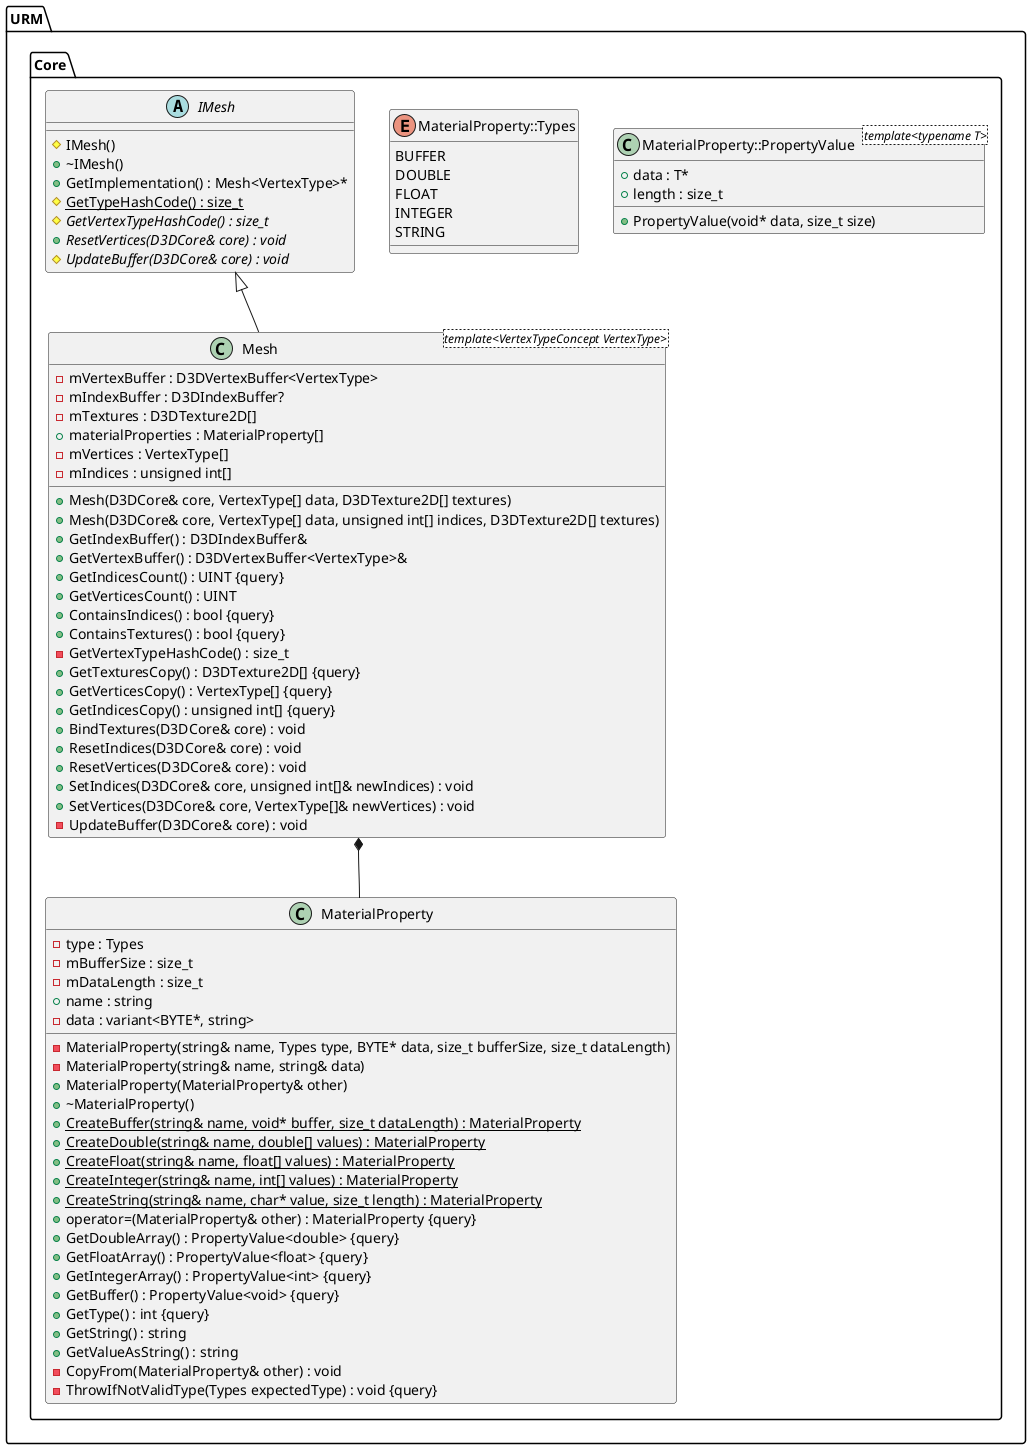
\includegraphics[width=\textwidth]{images/UML/mesh.png}
		\caption{Schemat klasy Mesh oraz klas wspierających.}
		\label{UML_Mesh}
	\end{figure}
	
		
	\vfill
	\clearpage
	
\subsection{Wczytywanie modeli}
	Funkcje pomocnicze ułatwiające wczytywanie modeli z pliku udostępnione zostały w ramach metod statycznych klasy \textbf{ModelLoader}. Metoda \textit{LoadFromFile()} jako argument otrzymuje ścieżkę do pliku modelu w obsługiwanym formacie, a następnie zwraca strukturę drzewową, której wierzchołkami są obiekty klasy \textbf{ModelLoaderNode}. Każdy wierzchołek zwracanego drzewa posiada macierz transformacji względem rodzica, listę mesh'y oraz wierzchołków przynależnych. Zachowywana zostaje oryginalna relacja transformacji między obiektami z wczytywanego pliku.
	Wraz z geometrią modelu wczytywane są także parametry metadanych do listy \textit{MaterialProperty} oraz przynależne do modelu tekstury. 
	
	Ze względu na ograniczenia API Direct3D na tym etapie koniecznym było założenie standardowego typu wierzchołków, za który przyjęty został typ \textit{VertexPositionNormalTexture}, oznaczony dalej przy pomocy mechanizmu type alias jako \textbf{ModelLoaderVertexType}.
	
	Moduł obsługuje wszystkie formaty plików wspierane przez bibliotekę assimp, których pełna lista dostępna jest na stronie biblioteki \cite{github:assimp:FileFormats}. Szczególna uwaga została położona na wsparcie najczęściej spotykanych formatów, takich jak DAE, FBX, glTF / GLB, OBJ czy STL.
	
	Diagram opisywanych struktur został przedstawiony na rys. \ref{UML_ModelLoader}.
		
	\begin{figure}[h!]
		\centering
		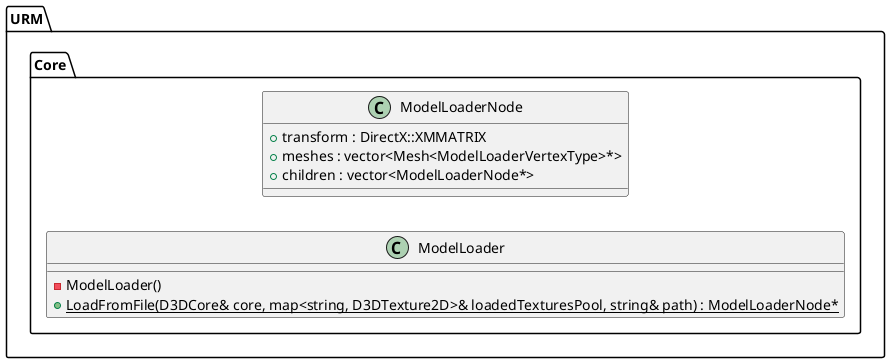
\includegraphics[width=\textwidth]{images/UML/modelloader.png}
		\caption{Schemat klasy statycznej ModelLoader wraz ze strukturą typu ModelLoaderNode.}
		\label{UML_ModelLoader}
	\end{figure}

\subsection{Tekstury}
	Kolejnym ważnym aspektem przy rysowaniu obiektów 3D są tekstury. Do reprezentacji ich dwuwymiarowych wersji powstała klasa \textbf{D3DTexture2D}, która przejmuje obowiązki wczytywania danych z pliku, utworzenia odpowiednich zasobów oraz zarządzania nimi. Istnieje także możliwość wczytania tekstury bezpośrednio z pamięci programu w formacie skompresowanym oraz nieskompresowanym.
	
	Do użycia z API D3D tekstury potrzebują także obiektu typu Sampler, który definiuje zachowanie próbkowania kolorów tekstury przy odczycie. Do ułatwienia tego zadania utworzona została klasa \textbf{D3DSampler}.
	
	Uproszczony schemat sekcji tekstur został opisany na rys. \ref{UML_Textures}.
	
	\begin{figure}[h!]
		\centering
		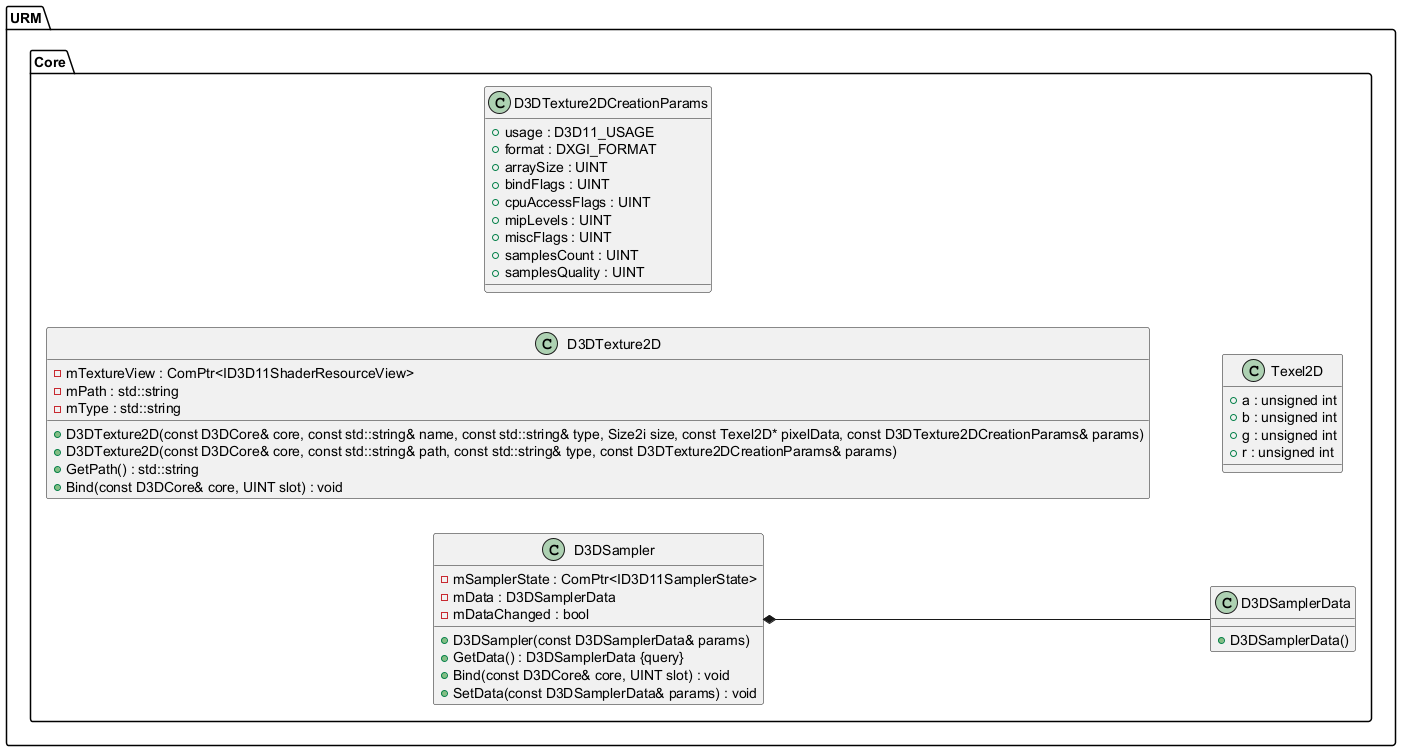
\includegraphics[width=\textwidth]{images/UML/texture.png}
		\caption{Schemat modułu tekstur.}
		\label{UML_Textures}
	\end{figure}
	
\subsection{Shader}
	Do reprezentacji segmentu programów cieniujących powstała abstrakcyjna klasa \textbf{Shader}, na podstawie której zaimplementowane zostały klasy \textbf{VertexShader} oraz \textbf{PixelShader}, służące odpowiednio do obsługi programów przetwarzania wierzchołków oraz wyliczania koloru pixeli. Oddają one do dyspozycji metody wczytywania z pliku w konstruktorze oraz przypisywania zawieranego przez nie programu jako aktywnego przy pomocy funkcji \textit{Bind()}.
	
	W ramach segmentu uwzględniony został także \textbf{D3DInputLayout}, służący jako warstwa abstrakcji nad układem danych wejściowych do shader'ów. Wykorzystuje on opisany w rozdziale \ref{SSMeshVertexTypeConcept} koncept \textit{VertexTypeConcept} do automatycznego dostosowania się do danych, a jego standardowa wersja wykorzystująca typ \textit{VertexPositionNormalTexture} oznaczona została jako \textbf{ModelLoaderLayout}.
	
	Diagram UML segmentu został przedstawiony na rys. \ref{UML_ShaderPipeline}.
	
	\begin{figure}[h!]
		\centering
		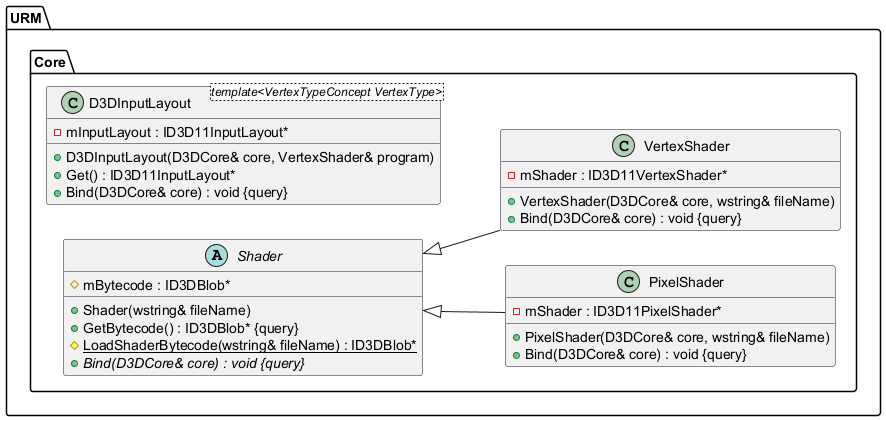
\includegraphics[width=\textwidth]{images/UML/shader.png}
		\caption{Schemat kompozycji klas Shader oraz D3DInputLayout.}
		\label{UML_ShaderPipeline}
	\end{figure}
	
	\vfill
	\clearpage
	
\subsection{Materiały}
	Programy cieniujące poza odniesieniem do używanego kodu w ramach klasy \textit{Shader} potrzebują także informacji o parametrach wyświetlanego obiektu, takich jak jego kolor, użyta tekstura i inne właściwości powierzchni.	Do przechowywania tych informacji utworzona została abstrakcyjna klasa \textbf{Material}, a także jej 2 standardowe implementacje - \textbf{MaterialSimple} oraz \textbf{MaterialPBR}, opisujące odpowiednio uproszczony model oświetlenia z danymi powierzchni w strukturze \textbf{MaterialSimpleData} i bardziej złożony mechanizm oparty o PBR, gdzie dane materiału znajdują się w \textbf{MaterialPBRData}.
	
	Każda implementacja klasy \textit{Material} musi zdefiniować metodę \textit{GetShader()}, która zwraca referencję do obiektu programu cieniującego. Dzięki temu każdy materiał może posiadać odrębny, różniący się od innych shader i w ten sposób rozszerzać działanie modułu poprzez utworzenie zewnętrznych implementacji. Możliwe jest także mieszanie różnych typów materiałów (a tym samym shader'ów), gdyż jest on przypisany do mesh'y, a nie globalnie.
		
	\begin{figure}[h!]
		\centering
		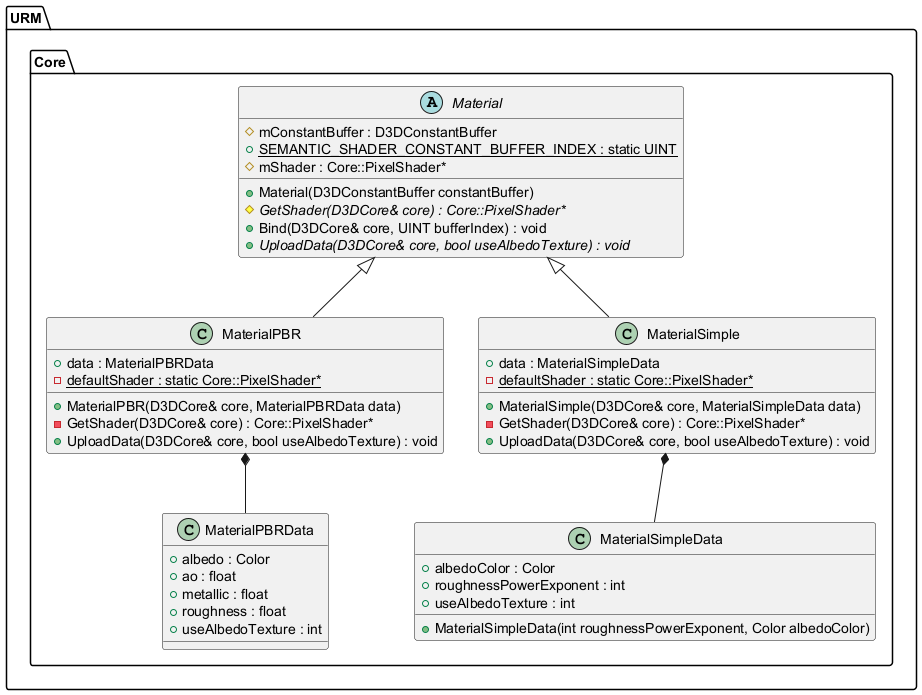
\includegraphics[width=\textwidth]{images/UML/materials.png}
		\caption{Schemat kompozycji abstrakcyjnej klasy Material oraz jej standardowych implementacji.}
		\label{UML_Material}
	\end{figure}
	
	\vfill
	\clearpage
	
\section{Engine}
	Podczas implementacji z przyczyn logistycznych zintegrowana została warstwa sceny oraz renderująca w ramach jednego projektu. Mimo tego zachowane zostało założenie budowy modularnej oraz możliwość użycia poszczególnych elementów bez konieczności korzystania z pozostałych na tym samym lub wyższym logicznie poziomie.
	
\subsection{Scene}
	Główna struktura zawierająca pełne informacje o rysowanej scenie, której diagram został przedstawiony na rys. \ref{UML_Scene}. Przechowuje ona współdzieloną referencję do głównego wierzchołka struktury obiektów, kamery ustawionej jako głównej, menadżera zasobów oraz struktury rdzeniowej \textit{(D3DCore)}. Posiada ona także listę odniesień do istniejących w scenie świateł oraz mesh'y, co pozwala na optymalizację ich rysowania ze względu na eliminację konieczności każdorazowego przechodzenia sceny w ich poszukiwaniu podczas procesu renderowania.
	
	\begin{figure}[h!]
		\centering
		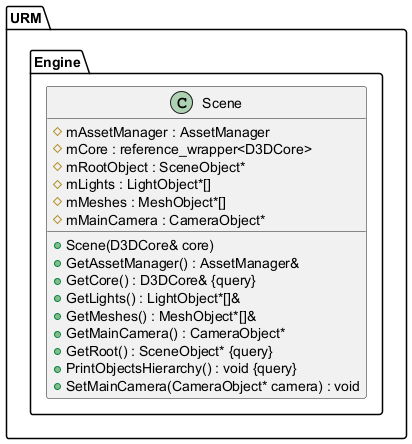
\includegraphics[width=\textwidth]{images/UML/scene.png}
		\caption{Schemat kompozycji klasy opisującej scenę.}
		\label{UML_Scene}
	\end{figure}
	
	
\subsection{Obiekt sceny}
	Klasa opisująca wierzchołek struktury drzewowej opisującej rysowany świat. Jest ona jednocześnie klasą bazową, z której dziedziczyć mogą obiekty implementujące wyspecjalizowane funkcjonalności. Posiada w swojej kompozycji odniesienie do sceny w której się znajduje, a także do \textit{"rodzica"} oraz listę \textit{"dzieci"} danego wierzchołka. 
	
	Ważnym elementem jest skomponowany obiekt klasy \textbf{Transform}, opisujący transformację przestrzenną obiektu w scenie. Przechowuje te informacje za pomocą macierzy transformacji, a także wyliczonych na jej podstawie wektory pozycji, skali oraz rotacji w dwóch wersjach - względem rodzica oraz globalnej. Do ich zmiany oddane zostały metody \textit{GetLocal\{Position/Rotation/Scale\}} do ustalania parametrów w przestrzeni lokalnej oraz \textit{Set\{Position/Rotation\}} do odmiany globalnej. Funkcje te wykonują automatyczną rekalkulację przestrzenną obiektu oraz jego dzieci. W ten sposób możliwe jest zachowanie relacji transformacji w hierarchii sceny bez konieczności zarządzania tym procesem z perspektywy programisty.
	
	Kompozycja oraz relacje między opisanymi klasami zostały pokazane na rys. \ref{UML_SceneObject}.
	
	\begin{figure}[h!]
		\centering
		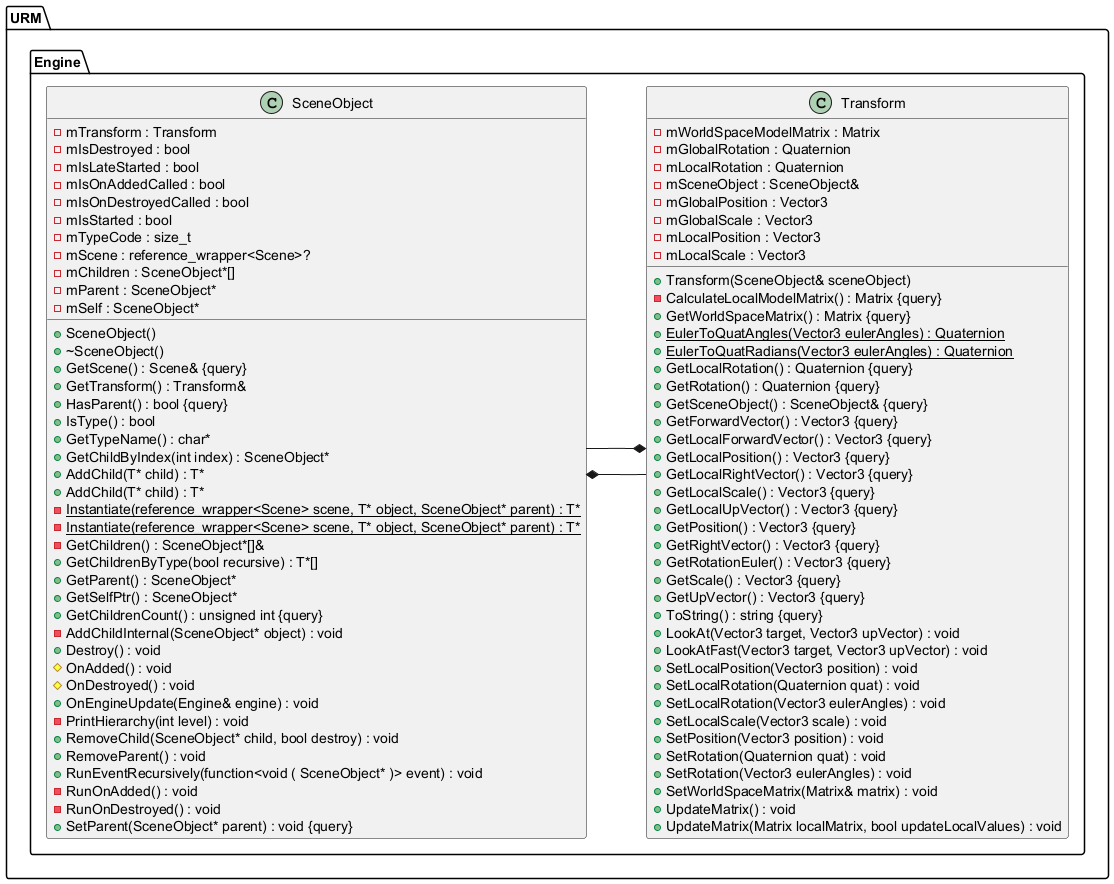
\includegraphics[width=\textwidth]{images/UML/sceneobject.png}
		\caption{Klasa obiektu sceny oraz transformacji.}
		\label{UML_SceneObject}
	\end{figure}
	
\subsection{Manager zasobów}
	Większość zasobów w ramach modułu jest automatycznie zarządzana przy pomocy inteligentnych wskaźników. Wczytywanie niektórych danych, takich jak modeli czy tekstur jest jednak czasochłonne i posiada nieunikniony narzut obliczeniowy. Przy wielokrotnym wykorzystaniu takich obiektów warto wprowadzić mechanizm typu cache, który przechowywać będzie referencje do już wczytanych elementów celem ich użycia zamiast ponownego ładowania od zera.
	
	Implementacją takiego mechanizmu w module jest \textbf{AssetManager}, przedstawiony na rys. \ref{UML_AssetManager}. Przechowuje on wczytane modele oraz tekstury w postaci słowników wykorzystujących typ std::map z C++ STL w celach optymalizacyjnych. Modele wczytane przy pomocy metody \textit{GetModel()} są automatycznie dodawane do cache'u, a każde kolejne wywołanie tej metody z tą samą ścieżką zwracać będzie już wczytany do pamięci model zamiast ponownego wczytywania i dekodowania z dysku.
	
	W niektórych przypadkach konieczne jest wyczyszczenie cache'u (na przykład przy zmianie sceny). Do tego celu oddana została metoda ClearAll(), która usuwa referencje do modeli i tekstur z managera. Nie są one jednak automatycznie zwalniane, gdyż referencje do nich nadal mogą istnieć w innych miejscach. Za ostateczne zwalnianie pamięci odpowiedzialny jest opisywany wcześniej mechanizm inteligentnych wskaźników.
	
	\begin{figure}[h!]
		\centering
		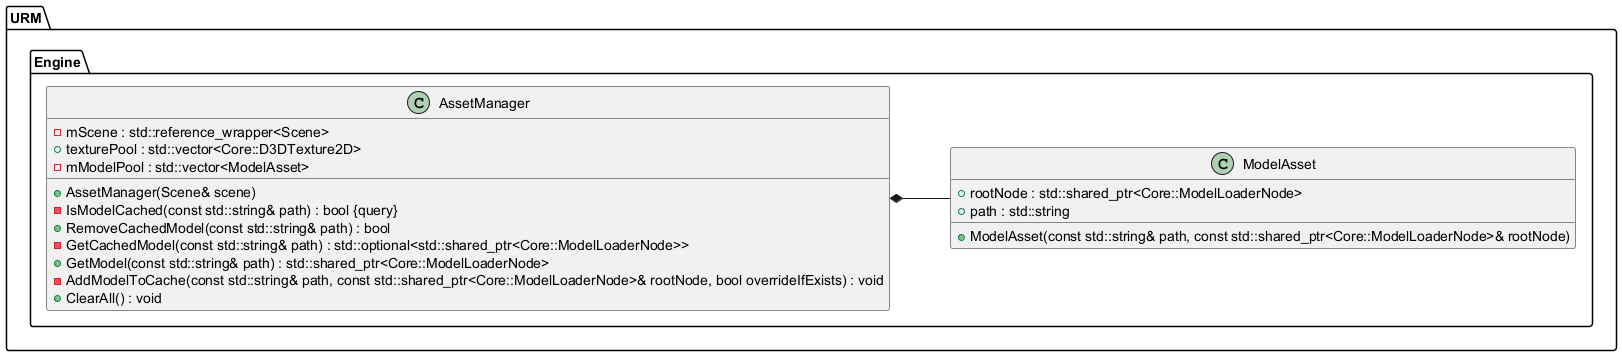
\includegraphics[width=\textwidth]{images/UML/assets.png}
		\caption{Diagram UML przestawiający schemat manager'a zasobów.}
		\label{UML_AssetManager}
	\end{figure}
	
	
\subsection{Obiekty modeli}
	Najważniejszym elementem w świecie programu do trójwymiarowej grafiki komputerowej są mesh'e oraz składające się z nich modele. W celu umieszczenia ich w hierarchii sceny i świata utworzone zostały klasy odpowiednio \textbf{ModelObject} oraz \textbf{MeshObject}, których schemat przedstawiony został na rys. \ref{UML_SceneObjects_Model}. Dla poprawienia czytelności diagramu typy parametrów konstruktorów zostały pominięte.
	
	\textit{ModelObject} odpowiedzialny jest za wczytanie modelu z pliku przy pomocy klasy \textit{AssetManager}, a następnie odpowiednie umieszczenie jego wierzchołków wraz z odpowiednimi transformacjami na scenie. Każdy pusty wierzchołek zostaje dodany jako obiekt klasy \textit{SceneObject}, a elementy zawierające mesh jako \textit{MeshObject} z zachowaniem odpowiedniej struktury między nimi.
	
	Po załadowaniu danych o geometrii z pliku wykonywana jest także próba odczytu parametrów przypisanego do niej materiału. Odpowiedzialna za to metoda \textit{TryDeduceMaterial(...)} analizuje elementy wczytanej w pierwszym etapie listy \textit{MaterialProperties}, z której wykonuje próbę dedukcji wspieranych parametrów materiału po ich nazwach. Mechanizm ten opiera swoje działanie o słownik materialPropertiesMap, zawierający mapę łączącą tekstową nazwę parametru zakodowaną w plikach modeli z obiektem typu \textbf{MaterialData}. Zawiera on informacje o spodziewanym typie z enum \textbf{MaterialProperties} oraz oczekiwanej liczbie elementów tablicy danych, dzięki której możliwa jest automatyczna weryfikacja poprawności wczytanego opisu i uniknięcie wyjścia poza zakres tablicy przy jego odczycie.
	
	Do poprawnego działania mesh wymaga odniesienia do obiektu rdzeniowego typu \textit{D3DCore}, którego pobranie możliwe jest dopiero gdy obiekt znajduje się na scenie. W związku z tym wczytanie modeli z pliku następuje dopiero w momencie dodania obiektu \textit{ModelObject} do świata, czyli w implementacji metody \textit{OnAdded()}, a nie przy tworzeniu instancji klasy.
	
	\begin{figure}[h!]
		\centering
		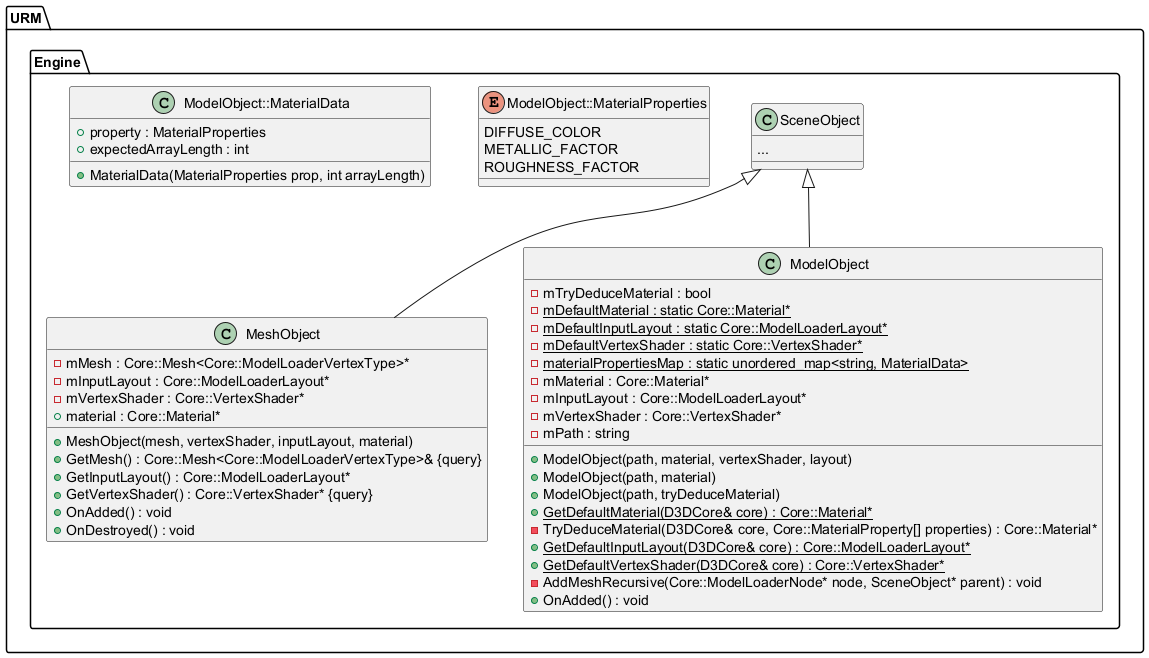
\includegraphics[width=\textwidth]{images/UML/sceneobjects_model.png}
		\caption{Obiekty sceny odpowiedzialne za modele, dziedziczące z klasy SceneObject.}
		\label{UML_SceneObjects_Model}
	\end{figure}

\subsection{Obiekt światła}
	Kolejnym zdefiniowanym jako element sceny obiektem jest przedstawiony na rys. \ref{UML_SceneObjects_Light} \textbf{LightObject}, reprezentujący wirtualne źródło światła. Zaimplementowane zostały 2 wersje oświetlenia - uproszczona oraz PBR, dzielące ze sobą wspólne parametry opisujące punkt oświetlenia:
	\begin{itemize}
		\item \textbf{Kolor (color)} - wartość opisująca składowe RGB źródła światła.
		\item \textbf{Parametr zaniku z odległością (attenuationExponent)} - pozawala na kontrolę siły zanikania intensywności światła z odległością. Przyjmuje on pozycję zmiennej w równaniu \(I = I_z / d^a\), gdzie \(I\) jest jasnością wynikową, \(I_z\) intensywnością źródła, \(d\) odległością od punktu źródłowego, a \(a\) wartością \textit{attenuationExponent}.
		\item \textbf{Intensywność komponentu otoczenia (ambientIntensity)} - opisuje poziom natężenia oświetlenia symulującego oświetlenie globalne. Składnik ten jest niezależny od kąta padania światła i zostaje nałożony uniwersalnie na wszystkie powierzchnie, uwzględniając jedynie odległość od źródła.
		\item \textbf{Intensywność komponentu rozproszonego (diffuseIntensity)} - natężenie światła odbitego niebezpośrednio. Przyjmuje wartość cosine z kąta między powierzchnią, źródłem światła, a kamerą.
		\item \textbf{Intensywność komponentu wziernikowego (specularIntensity)} - moc bezpośredniego odbicia światła, bezpośrednio zależnego od kąta padania oraz parametrów materiału.
		\item \textbf{Intensywność w trybie PBR} - ze względu na swoją charakterystykę przy kalkulacjach opartych o PBR większość sceny sprawia wrażenie mniej oświetlonej od trybu uproszczonego. Aby zapobiec takiemu zachowaniu i zbliżyć poziom jasności obu trybów wprowadzony został opisywany parametr, będący mnożnikiem intensywności światła ignorowanym w uproszczonej wersji.
	\end{itemize}
	
	Symulacja oświetlenia jest szybko rozwijającym się tematem w dziedzinie grafiki trójwymiarowej, a modularna forma implementacji opisywanej klasy oraz programów cieniujących w ramach \textit{Material} pozwala na doimplementowanie bardziej zaawansowanych technik w razie zaistnienia takiej potrzeby.
	
	\begin{figure}[h!]
		\centering
		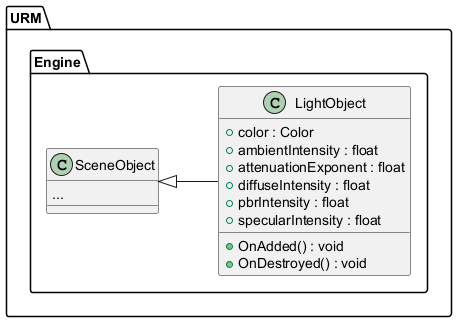
\includegraphics[width=\textwidth]{images/UML/sceneobjects_light.png}
		\caption{Reprezentacja punktu światła w wirtualnej przestrzeni.}
		\label{UML_SceneObjects_Light}
	\end{figure}
	
\subsection{Obiekt kamery}
	Samo rysowanie sceny byłoby mało użyteczne, jeśli nie istniałby sposób aby się po niej poruszać. Do tego celu oddana została klasa \textbf{CameraObject}, której funkcjonalność opiera się na abstrakcji nad złożonymi transformacjami sceny w formie prostego obiektu w przestrzeni sceny. Przechowuje ona informacje o parametrach rysowania, takich jak dystans odcięcia bliskiego \textit{(mNearPlane)} oraz dalekiego \textit{(mFarPlane)}, a także pola widzenia w formie kąta pionowej składowej \textit{(mFov)}. Na ich podstawie możliwe jest obliczenie macierzy projekcji \textit{(CalculateProjectionMatrix())} oraz widoku \textit{(CalculateViewMatrix())}, wykorzystywanych w dalszej części do transformacji rysowanego świata.
	
	Bardzo częstym sposobem podejścia do tematu kamery w aplikacjach grafiki komputerowej jest wersja sterowana przez użytkownika. Implementacja takiej funkcjonalności znajduje się w klasie \textbf{FlyCameraObject}, która automatyzuje odczytywanie wejścia użytkownika z klawiatury i na ich podstawie oraz parametrów prędkości porusza i obraca wirtualną kamerą w świecie aplikacji.
	
	Schemat opisywanych klas został pokazany na rys. \ref{UML_SceneObjects_Camera}.
	
	\begin{figure}[h!]
		\centering
		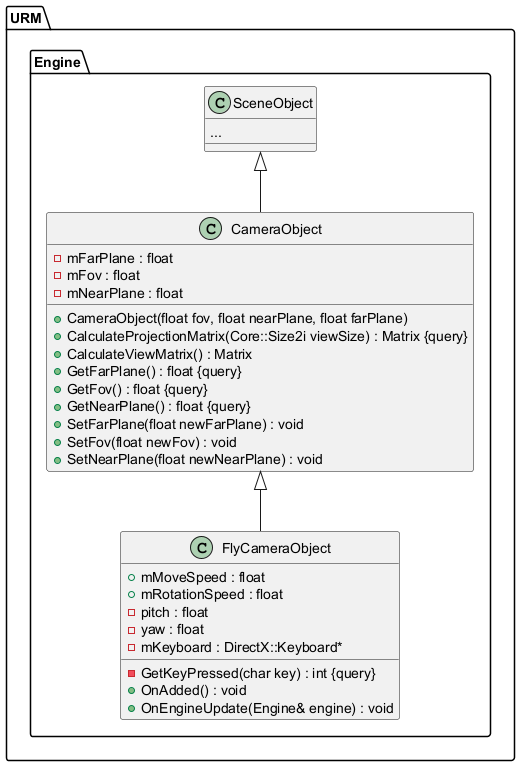
\includegraphics[width=\textwidth]{images/UML/sceneobjects_camera.png}
		\caption{Klasa reprezentująca wirtualną kamerę renderującą scenę oraz jej wersja sterowana przez użytkownika.}
		\label{UML_SceneObjects_Camera}
	\end{figure}
	
\subsection{Engine}
	Klasa silnika, spajająca większość opisanych do tego momentu funkcjonalności modułu.
	
	\begin{figure}[h!]
		\centering
		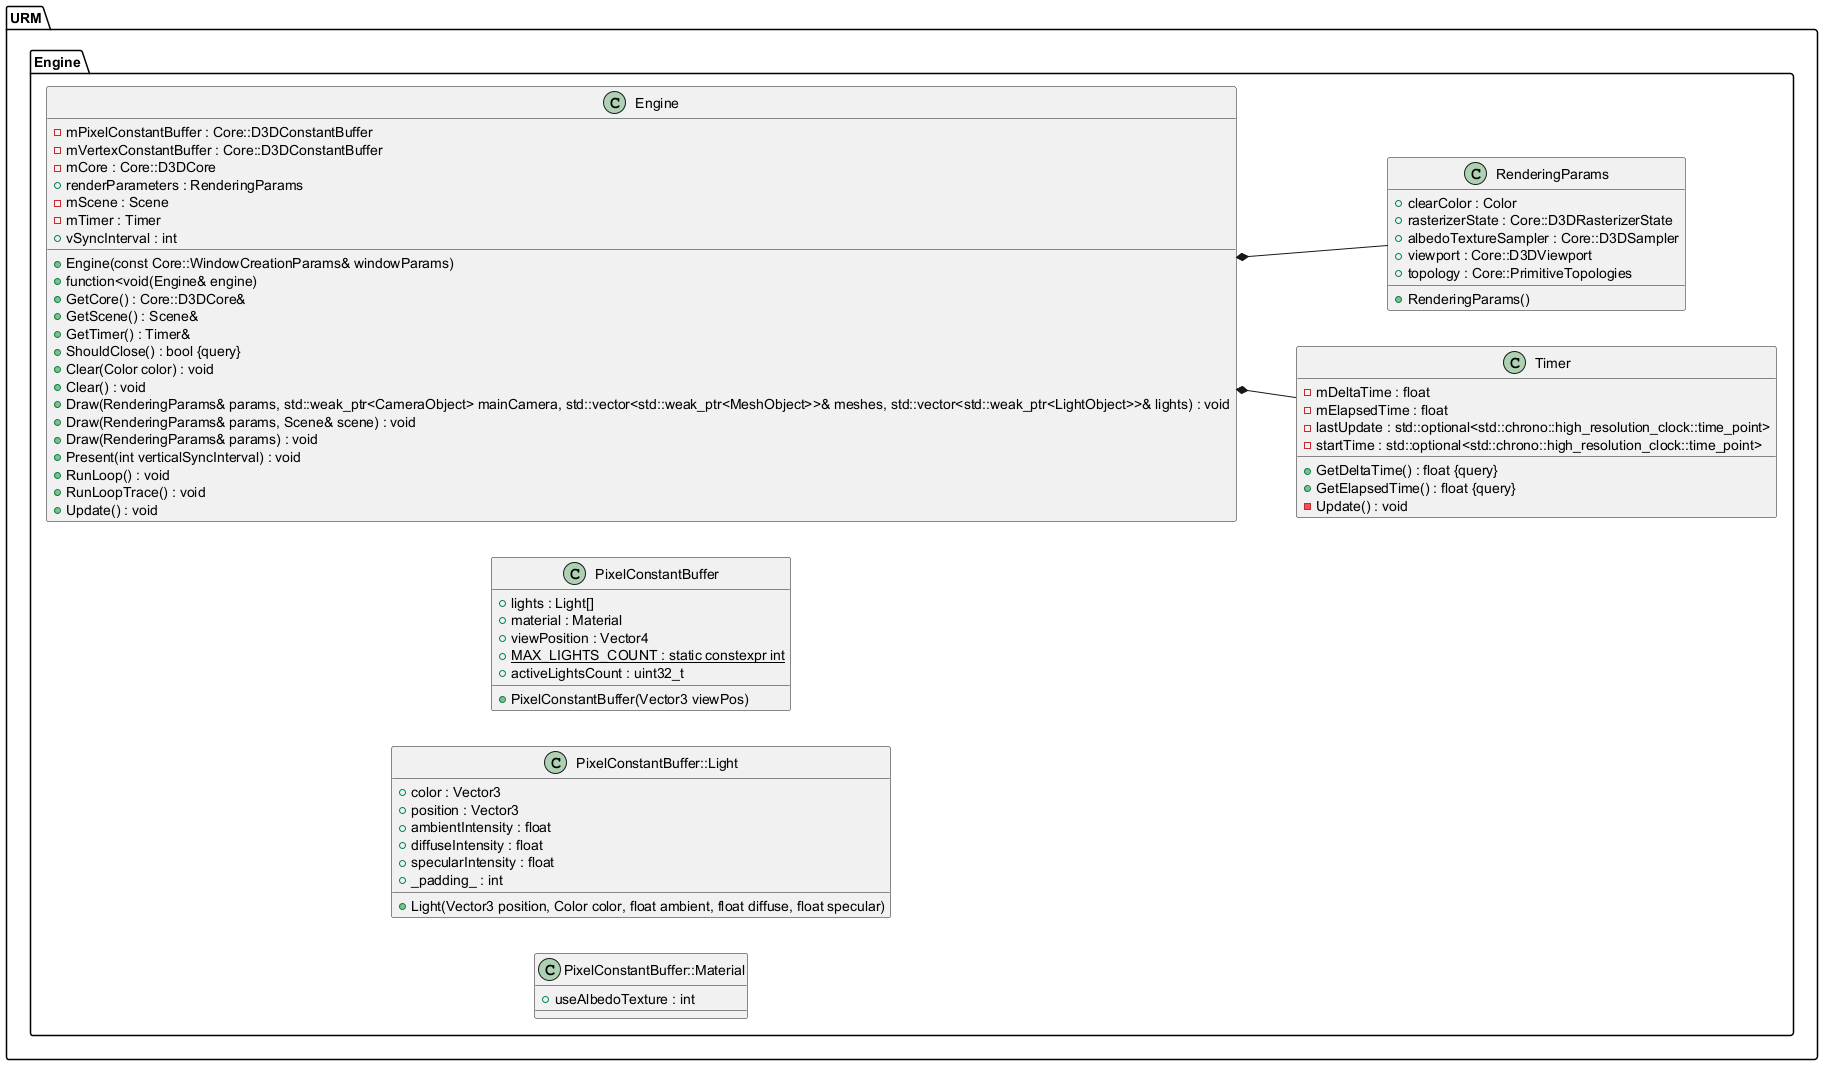
\includegraphics[width=\textwidth]{images/UML/engine.png}
		\caption{Klasa reprezentująca wirtualną kamerę renderującą scenę oraz jej wersja sterowana przez użytkownika.}
		\label{UML_Engine}
	\end{figure}